\pattern{Mediator} 
\begin{summary} 
    A {\bf mediator} is an object that encapsulates a web of relations or
    interactions between sets of other objects, acting as an intermediary which
    decouples dependent objects. This allows objects to communicate without
    referring to each other explicitly. Instead, objects send requests to the
    mediator, which processes and directs them to the appropriate subject. 

    Mediator patterns are best suited for situations where a set of objects
    communicate in complex ways. Multiple unstructured interdependencies
    creates difficulty in understanding the process of events and the ability
    to reuse objects.
\end{summary}

\comparison{\begin{itemize}
        \item Low coupling: Since objects communicate with a mediator instead
            of directly, they are unaware of other component's implementations. 
        \item Maintainability: adding, deleting, and modifying components and
            relations is easy since components are encapsulated. By separating
            relations between classes and grouping them in a different class,
            any change to one component will not affect the rest of the code.
        \item Code reuse: Since objects communicate in a common shared way
            with a central mediating object, code can be reused between
            objects. 
        \item Flexibility: Mediators model the inter-relationships of
            objects to allow modification and extension of these
            inter-relationships through subclassing and allows flexibility.
        \item Readability: Centralized communication between objects can make
            it clearer when objects are communicating, and with which other
            objects. 
\end{itemize}

}{\begin{itemize}
        \item Readability: The mediator can become ``God object'' that knows
            too much or does too much. This can lead to a complicated and hard
            to understand system.
        \item Maintainability: The system can become counterproductive, 
            ineffective, and risky if the mediator controls too much, or if
            objects communicate in a complex and poorly defined way.
\end{itemize}
}% END comparison

\begin{nfps}
\item[Complexity] It increases developer understanding needed to work with
    the components. Individual components have clearer interactions, which are
    defined through a standard interface. The {\sc Mediator} class that
    centralizes communication creates an easy way to see all relations.
\item[Scalability] Low coupling due to the lack of dependencies between
    components allows for new components/relations which will not affect
    existing components/relations. The addition of components from other
    applications just requires a new mediator. 
\end{nfps}

\subsubsection{Example}
When texting your friend, you are not making a direct connection between your
phones. Many mediators are involved in this process. Bits that make up your
message is sent to a cell tower closest to you. The switching service is then
handled by your carrier which helps establish the connection to your friend on
your behalf. The message is then passed to the cell tower closest to your
friend. Finally, the message appears on your friend’s phone. In this scenario,
your carrier is the main mediator.

\begin{center}
    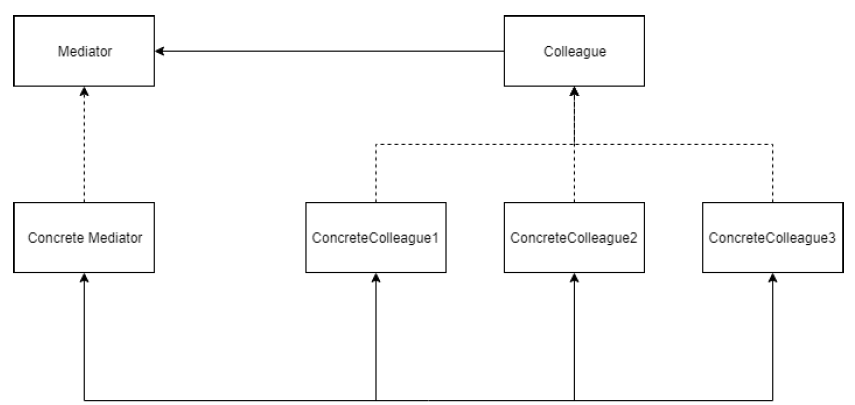
\includegraphics[width=0.4\textwidth]{./mediator1}
    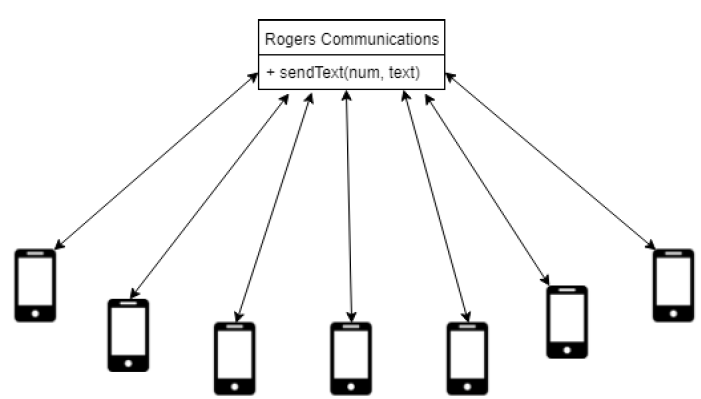
\includegraphics[width=0.4\textwidth]{./mediator2}
    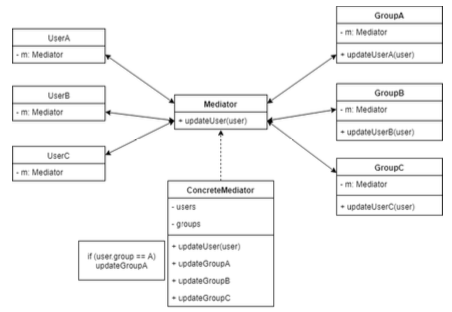
\includegraphics[width=0.4\textwidth]{./mediator3}
\end{center}
